\documentclass[11pt]{scrbook} %% 	arirang-kotex.tex :: mito / nyamcoder
\usepackage[hanja]{kotex}
\usepackage{graphicx}	% bildeinbindung
\renewcommand\chaptermark[1]{\markboth{\textsf{#1}}{}} % damit nur der chaptertitel erscheint 
\usepackage{wasysym}	% --> \twonotes 
\usepackage{titlesec}
\renewcommand\thesection{(\arabic{section})\,}
\titleformat{\section}{\centering\sf\bfseries\Large}{}{0em}{\fbox}
\usepackage{scrpage2}	% nicht nur für KOMA, scrguide-137ff 
\setheadsepline{.2pt} % [Anweisungen] scrguide-146 ; [text] linienlänge --> hier auf textbreite ==  standard 
\pagestyle{scrheadings}
\ihead{\leftmark}
\lehead{\twonotes\quad\rightmark}
\rohead{\rightmark\quad\twonotes}
\ofoot{\pagemark}		% scrguide-137ff 
\refoot{\upshape\ksKSTHE~\thepart~\partname}
\lofoot{\upshape 우리 음악의 발달사}
\renewcommand{\partpagestyle}{empty} % fkt nicht ohne scr(book), scrguide-94ff
\renewcommand{\chapterformat}{\ksKSTHE~\thechapter~\chaptername\qquad} 
\renewcommand{\chapterpagestyle}{empty}	% scrguide-94ff 
\newcommand\sans{\sffamily\SetAdhocFonts{utgt}{}}
 
\begin{document}
\tableofcontents\thispagestyle{empty}
\pagebreak
\part{우리 음악의 발달사}
\chapter{民謠}	% 민요
\pagebreak
\section{아리랑}
\renewcommand\theenumi		{\ogana{enumi}} 
\renewcommand\labelenumi	{\textbf\theenumi}
\renewcommand\theenumii		{\Hnum{enumii} 절}	
\renewcommand\labelenumii	{\sans\theenumii\quad}
\renewcommand\labelitemi	{\quad $\circ$}
\begin{enumerate} 
\linespread{.97}\selectfont
\item \textbf{멜로디}\\[.5em]
\hspace*{13mm}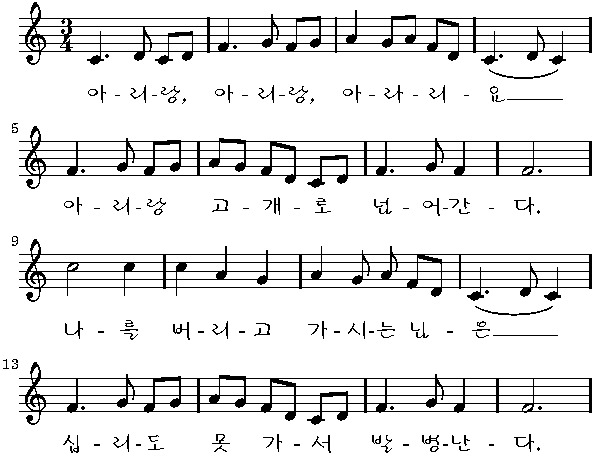
\includegraphics[height=7.5cm]{./staff/lily-db16faf4.pdf}
\item \textbf{노랫말}
\begin{sans}
\begin{enumerate}
		\item 아리랑, 아리랑, 아라리요,\\
				아리랑 고개로 넘어간다.\\
				나를 버리고 가시는 님은\\
				십리도 못가서 발병난다.
		\item 청천하늘엔 별도 많고\\
				우리네 가슴엔 꿈도 많다
		\item 저기 저 산이 백두산이라지\\
				동지 섣달에도 꽃만 핀다
\end{enumerate}
\end{sans}
\item \textbf{여러 가지 아리랑}
	\begin{itemize}
		\item 본조(本調) 아리랑
		\item 정선 아리랑
		\item 강원도 아리랑
		\item 밀양 아리랑
		\item 진도 아리랑 등
	\end{itemize}
\item \textbf{기타}
	\begin{itemize}
		\item 1926년	\textbf{나운규(羅雲奎  Na Woon-gyu)}의  영화 ``아리랑''에 대해서 \textsf{한국의 영화계: 무성 영화의 황금시대} 참조 % \pageref{sec:film-silent}페이지를 참조
		\item 1967년 \textbf{John Barnes Chance}의 ``Variations on a Korean Folk Song''에 대해서 \textsf{클래식} 참조 % \pageref{sec:classic}페이지를 참조
	\end{itemize}		
\item 그 이외의 텍스트 \dots
%% 계획: 
%%\section{클래식}
%%\label{sec:classic}
%%\chapter{한국의 영화계}
%%\section{무성 영화의 황금시대}
%%\label{sec:film-silent}
%%\section{남한의 영화}
%%\section{북한의 영화}
%%\chapter{한류 열풍}
%%\section{대한민국의 텔레비전 드라마}
%% 등		% see \part{한국 영화}
\end{enumerate}
\end{document}


%%%%%%%%%%%%%%%%%%%%%%%%%%%%%%%%%%%%%%%%%%%%%%%%%%%%%%%%%%%%%%%%%%%%%%%%%%%

compilation order
=================

1. staff compilation (see ./staff/arirang-sheet.tex)

* example lilypond-book output

% lilypond wird ausgeführt...GNU LilyPond 2.10.33
% »snippet-map.ly« wird verarbeitet
% Analysieren...
% »arirang-cjk-test.tex« wird verarbeitet
% Analysieren...
% Interpretation der Musik...[8][16]
% Vorverarbeitung der grafischen Elemente...
% Zeilenumbrüche werden berechnet... 
% Drawing systems... 
% lily-2f55749803-systems.tex wird geschrieben...
% lily-2f55749803-systems.texi wird geschrieben...
% Layout nach »lily-2f55749803-1.eps« ausgeben...
% Layout nach »lily-2f55749803-2.eps« ausgeben...
% Layout nach »lily-2f55749803-3.eps« ausgeben...
% Layout nach »lily-2f55749803-4.eps« ausgeben...
% Layout nach »lily-2f55749803.eps« ausgeben...
% Warnung: keine Musik in der Partitur gefunden

% arirang-cjk-test.tex kompilieren...
% »arirang-cjk-test.tex« wird geschrieben...
% Schriftarten werden nach arirang-cjk-test.psfonts geschrieben...

 --> import processed pdf into this file (arirang-kotex.tex)


2. main document compilation (double for table of contents)

$ pdflatex arirang-kotex && pdflatex arirang-kotex 
